% Copyright (c) 2026 Geovana Neves. Licensed under CC BY 4.0 (https://creativecommons.org/licenses/by/4.0/). See LICENSE-AND-AUTHORSHIP.md.
%
% guide/fsi/text/07b-xprop-titanium.tex
%
% Worked example 4: the public XPROP rotor as solid titanium, the stiffness
% gain varied, against rigid blades. Every number is the campaign's own
% record, run natively on 26.124. The figures in 06-fsi/figures/ are that
% campaign's, copied as is. No geometry of the rotor is stated here: it is
% cited by its public record.
%
% What this example must never let a reader believe: that the in-run coupled
% route produced these numbers. It did not; with the earlier command sequence
% it failed on this rotor at the first coupling call, and the sweep was
% obtained by route B, a partitioned static iteration on the package's own
% structural chain. The second frame says so before any result is shown.
%
% No em dashes and no en dashes.

\section{Worked example: the XPROP rotor in titanium}

\begin{frame}{Example 4: the XPROP rotor as solid titanium}
\begin{columns}[T]
\begin{column}{0.55\textwidth}
\begin{itemize}\scriptsize
  \item The XPROP rotor [2], six blades, \(J = 1.70\), 473.2 rev/min,
        Mach 0.144; unsteady, 10\(^\circ\) per step, four revolutions, far field
        5 layers; build 26.124 [3].
  \item The blades are \textbf{solid Ti-6Al-4V} from the package database:
        \(\rho\) 4430 kg/m\(^3\), \(E\) 113.8 GPa, \(G\) 44.0 GPa (tabulated),
        \(\nu\) 0.342; sections calculated from the blade contours
        (\code{inputs/fsi/f001.toml}, calculated mode).
  \item The \textbf{stiffness gain} \(K\) scales EI and GJ together through the
        matrix: \code{FSI\_BENDING\_STIFFNESS\_N\_M2\_FACTOR} and
        \code{FSI\_TORSION\_STIFFNESS\_N\_M2\_FACTOR} = 0.5, 1.0, 2.0; mass and
        inertia unchanged. Provenance records both with origin \code{matrix}.
  \item The comparison: the same rotor with \textbf{rigid blades}.
\end{itemize}
\end{column}
\begin{column}{0.41\textwidth}
\begin{ftsevidence}[The matrix, in one line each]
\scriptsize
rigid: no \code{FSI} column\\
titanium: \code{FSI: f001}, both factors \(= K\)\\[2pt]
One structural file, three rows: the gain is a matrix variable, never a new
input file.
\end{ftsevidence}
\end{column}
\end{columns}
\fsicampaign{the campaign's record}
\end{frame}

\begin{frame}{Example 4: solved by route B, because the coupled route failed here}
\begin{columns}[T]
\begin{column}{0.50\textwidth}
\begin{ftslimit}[What the earlier command sequence did here]
\scriptsize
The three coupled rows stopped at the first coupling call: the solver reported
the RBF weights singular in the LU decomposition and exited. The node file
imported once per blade frame leaves coincident nodes on 26.124 for a rotor of
more than one blade. It was a defect of that command sequence; none of those
rows is a result.
\end{ftslimit}
\end{column}
\begin{column}{0.46\textwidth}
\begin{itemize}\scriptsize
  \item \textbf{Route B} instead (Part 1): the package's own chain
        (\code{to\_elastic\_axis}, \code{solve\_rotating\_static}) on the native
        sectional loads gives flap \(w(r)\) and twist \(\theta(r)\).
  \item Every mesh vertex moves about the elastic axis by that \(w\) and
        \(\theta\); the solver reruns the deformed rotor as the baseline.
  \item Stop: tip flap changes by less than 1\,\% and tip twist by less than
        0.005\(^\circ\) between two structural solutions.
  \item Control: a zero deformation through the same pipeline reproduces the
        rigid rotor to \(2.4\times10^{-5}\) in thrust.
\end{itemize}
\end{column}
\end{columns}
\fsicampaign{\code{fsi\_route\_diagnostic.json}}
\end{frame}

\begin{frame}{Example 4: what the earlier sequence did, and what changed}
\relax % a body opening with a brace group would be read as the frame subtitle
{\ftstablesize\renewcommand{\arraystretch}{1.08}
\begin{tabular*}{\linewidth}{@{\extracolsep{\fill}}llccc@{}}
\toprule
configuration on 26.124 & earlier planner & loop runs & deforms & rotation \\
\midrule
six blades, product route & accepted & no: RBF singular & & \\
one blade, no symmetry, product route & accepted & yes, 81 calls & \textbf{no} & yes \\
one blade, periodic copies (a sector) & refused & & & \\
one blade, 5 cm prescribed, rotating & (probe) & yes & \textbf{no} & yes \\
one blade, 5 cm prescribed, no motion & (probe) & yes & \textbf{no} & \\
fixed wing, steady & refused & callback never called & \textbf{no} & \\
fixed wing, unsteady, 0.2 m prescribed & refused & yes, every step & \textbf{no} & \\
fixed wing, unsteady, coupled beam & refused & yes, 30 of 30 & \textbf{no} & \\
\bottomrule
\end{tabular*}}
\par\vspace{2mm}
\begin{itemize}\scriptsize
  \item With no motion at all, a 0.2 m bend and a 5\(^\circ\) twist leave the loads
        identical to every printed digit: the displacement never reaches the
        aerodynamic surface, and motion is not the cause.
  \item Scope: the earlier command sequence, on 26.124. This version builds the
        nodes inside the blade and assigns the surface by its boundary
        identifier; with them a blade held still in a turning free stream maps
        and deforms (the \code{qsteady\_rotor} sector), while a turning blade
        is still deformed in its un-turned position, so \code{unsteady\_rotor}
        with FSI is refused [4].
\end{itemize}
\fsicampaign{\code{fsi\_wing\_probe.json}; \code{fsi\_route\_diagnostic.json}}
\end{frame}

\begin{frame}{Example 4: performance against the stiffness gain}
\centering
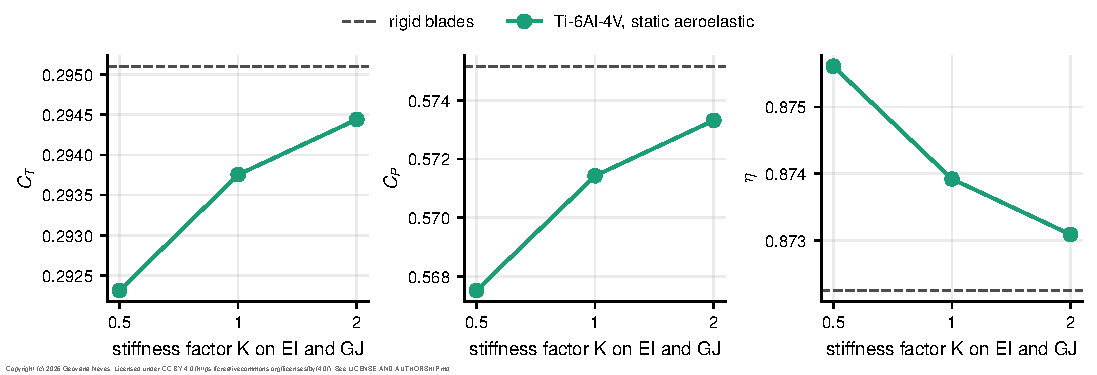
\includegraphics[width=0.97\linewidth]{figures/fsi_xprop_performance_vs_stiffness.pdf}
\par\vspace{1mm}
{\ftstablesize\renewcommand{\arraystretch}{1.05}
\begin{tabular*}{0.92\linewidth}{@{\extracolsep{\fill}}lrrrrrr@{}}
\toprule
case & \(T\) [N] & \(C_T\) & \(C_P\) & \(\eta\) & \(\Delta C_T\) [\%] & \(\Delta\eta\) [pts] \\
\midrule
rigid blades & 2078.0 & 0.2951 & 0.5752 & 0.8723 & & \\
Ti, \(K = 2.0\) & 2073.3 & 0.2944 & 0.5733 & 0.8731 & \(-0.23\) & \(+0.08\) \\
Ti, \(K = 1.0\) & 2068.4 & 0.2938 & 0.5714 & 0.8739 & \(-0.46\) & \(+0.17\) \\
Ti, \(K = 0.5\) & 2058.3 & 0.2923 & 0.5675 & 0.8756 & \(-0.95\) & \(+0.34\) \\
\bottomrule
\end{tabular*}}
\fsicampaign{\code{fsi\_xprop\_comparison.csv}}
\end{frame}

\begin{frame}{Example 4: how the blade deforms}
\centering
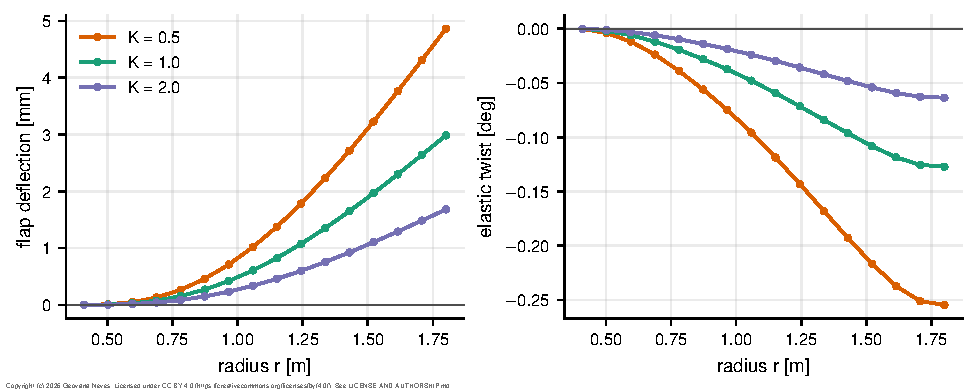
\includegraphics[width=0.80\linewidth]{figures/fsi_xprop_spanwise_deflection.pdf}
\par\vspace{1mm}
\begin{itemize}\footnotesize
  \item The elastic twist is \textbf{nose down} and scales as \(1/K\): it unloads
        the outer blade, so thrust and power fall and efficiency rises.
  \item The flap scales \textbf{less} than \(1/K\) (tip 1.68, 2.98, 4.86 mm):
        centrifugal tension stiffens the blade in flap, as the rotating beam says.
\end{itemize}
\fsicampaign{\code{fsi\_xprop\_spanwise\_deflection.pdf}}
\end{frame}

\begin{frame}{Example 4: convergence, and what the example establishes}
\centering
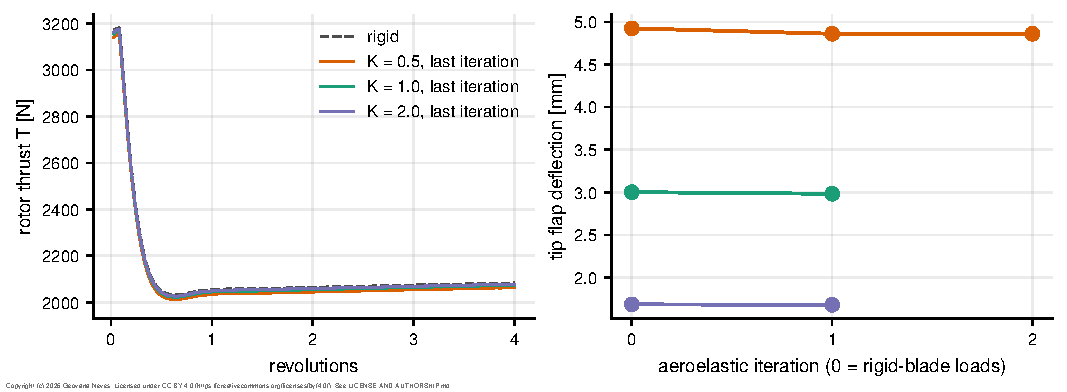
\includegraphics[width=0.66\linewidth]{figures/fsi_xprop_convergence.pdf}
\par\vspace{1mm}
\begin{columns}[T]
\begin{column}{0.48\textwidth}
\begin{itemize}\scriptsize
  \item One or two aeroelastic iterations suffice; the one-way answer (rigid-blade
        loads) is already within 1.3\,\% of the coupled flap.
  \item The change against rigid is stable to about 0.01 points over revolutions
        2 to 4.
\end{itemize}
\end{column}
\begin{column}{0.48\textwidth}
\begin{ftslimit}[What it does not establish]
\scriptsize
Native two-way coupling; dynamics (the iteration is static); absolute \(C_T\)
better than 0.45\,\% (thrust still rises that much per revolution). No spinner
or nacelle: rigid thrust 3\,\% below the same case run with them.
\end{ftslimit}
\end{column}
\end{columns}
\fsicampaign{\code{fsi\_xprop\_convergence.pdf}}
\end{frame}
